%Die Angabe des schlauen Spruchs auf diesem Wege funtioniert nur,
%wenn keine Änderung des Kapitels mittels den in preambel/chapterheads.tex
%vorgeschlagenen Möglichkeiten durchgeführt wurde.
\chapter{Problem Definition and Feature Selection}
\label{chap:chapter4}
%\vspace{-3cm}
%\vspace{2cm}
There are number of methods to separate permanent faults from non-recurring faults as explained in section ~\ref{sec:secfc}.However available techniques do not separate faults as permanent, transient and intermittent. This is of particular importance from point of view of reducing yield loss, by including chips which showed only transient behavior. Also, if faults can be categorized into these categories, then it gives an additional information to designer about the underlying fault, so that additional optimization of yield can be achieved. 

The classification approaches explained in section~\ref{sec:secfc} are mostly rule or heuristic based (e.g. threshold value in $\alpha$-counting techniques) and these heuristics or rules will change every time technology is node to lower nodes, hence these rules become obsolete over time. An elaborate analysis is required to update these rules for every product and technology.

Generally speaking, when an intermittent fault occurs in a system, its activation rate is higher than transient fault rate \cite{Bondavalli2000}. However, as systems are moving to lower technology nodes, transient faults are also on the rise, as explained in section~\ref{sec:secft}. Hence with traditional techniques, it becomes difficult to separate transients from intermittent using $\alpha$-count, as the fault rates for these two types of faults become close to each other.

This calls for an automated and adaptive approach which is independent on product and technology and can classify faults as intermittent, transient and permanent. 

\section{Machine learning approach for fault classification}

Machine learning has been used in wide variety of classification applications with reasonable accuracy \cite{Pang2002,Nguyen2008,Sebastiani2002, Kotsiantis2007}. As explained in chapter~\ref{chap:chapter3}, machine learning is used when it is not practical to arrive at rules by looking at data. Machine learning algorithms can be implemented as \enquote{black-box} approach for classification and all user needs to do is adjust few parameters, depending on machine learning algorithm used. Even parameter searching can be automated and user can fine-tune them for further improvement in accuracy \cite{Hsu2003, Castillo2000}. This makes machine learning a practical and automated approach when large amount of data is available.

Once a feature set is fixed and required parameters are decided, machine learning algorithms analyze the data to set up a classification model. When a technology node is updated one might have to change the database and train the algorithm again, but the training algorithm takes care of feature space and classification rules, making machine learning approaches adaptive.

We are going to use as supervised learning as aready explained in section~\ref{sec:secmltypes}. Figure~\ref{fig:mlsteps} explains basic steps for such classification.

\begin{figure}[h]
  \begin{center}
    \captionsetup{justification=centering}
    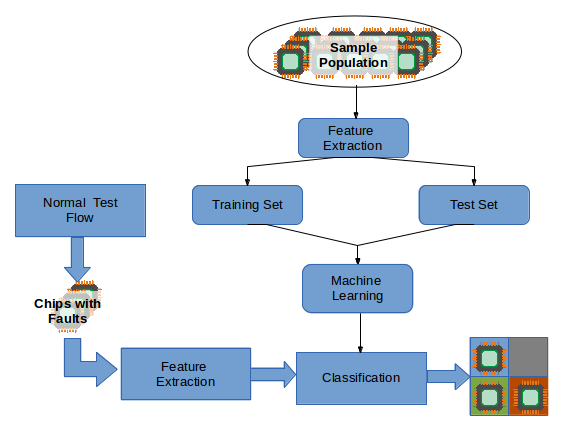
\includegraphics[scale=0.75]{figures/mlsteps.png}
    \caption{Classification of VLSI chips uning machine learning}
    \label{fig:mlsteps}
  \end{center}
\end{figure}

First step in designing a machine learning system for classification is to decide on the features that can be efficiently classify the data. Selection of proper features has the most impact in accuracy of any classifier \cite{Michie1994}. Next step is to design algorithms to extract features from input data. This is explained in section~\ref{sec:secfs} of this chapter. Then we generate sample population and decide on which machine learning algorithm is to be used, covered in next chapter.

\section{Feature Selection}
\label{sec:secfs}
To begin with feature selection, it is first important to take a look at all the behavioral chatacteritics of different types of faults,covered in chapter~\ref{chap:chapter2}. Table~\ref{tab:charfaults} summerises all important charecterisics to be considered for selection of features. Rest of the section describes features that were selected and algorithms for extraction of those features.

{%
\newcommand{\mc}[3]{\multicolumn{#1}{#2}{#3}}
\begin{table}[H]
 \begin{center}
  \captionsetup{justification=centering}
  \begin{tabular}{lp{4cm}p{4cm}p{4cm}}
    \mc{1}{c}{\textbf{Characteristic}} & \mc{1}{c}{\textbf{Permanent faults}} & \mc{1}{c}{\textbf{Intermittent faults}} & \mc{1}{c}{\textbf{Transient faults}}\\ \hline
    Affected outputs & Affects same set of output pins & Affects same set of output pins & Affects any of primary outputs\\
    Reproducibilty & Reproducible for same test vector & Sometimes reproducible for same test vector depending upon the error activation rate & Not preproducible\\
    Location on chip & Localized to a fault location & Localized to a fault location & Can affect any location on chip\\
    Fault behaviour & Deterministic & Deterministic & Non-deterministic \\ \hline
  \end{tabular}
  \caption{Characteristics of faults in VLSI systems}
  \label{tab:charfaults}
 \end{center}
\end{table}
}%

\subsection{Reproducibility of fault}
We define reproducibility of fault pattern during multiple test runs as maximum number as maximum number of occurance of same faulty output pattern for a fixed input pattern denoted by $\epsilon$. 

\begin{figure}[h]
  \begin{center}
    \captionsetup{justification=centering}
    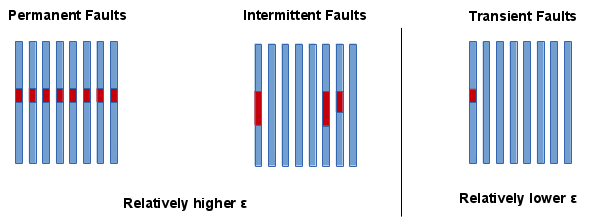
\includegraphics[scale=1.00]{figures/epsilon.png}
    \caption{Expected behavior of $\epsilon$ for different faults}
    \label{fig:epsilon}
  \end{center}
\end{figure}

Algorithm~\ref{alg:epsilon} explains extraction of $\epsilon$. It takes expected output pattern and actual output patterns as inputs. It then checks if any of output patterns was faulty and it calculates maximum occurances of every faulty pattern for given input pattern and stores in into array. Final value of $\epsilon$ is maximum value of in this array.

\begin{algorithm}[H]
  \caption{Algorithm to evaluate $\epsilon$}
  \label{alg:epsilon}
  \begin{algorithmic}
 \Procedure{ComputeEpsilon}{Expected output pattern array (EX), Array of output pattern array for all test runs (OP)}
 \State $\epsilon$[size(EX)] $\leftarrow$ 0\;
 \State Index $\leftarrow$ 0\;
 \While{Index $<$ size(EX)}
  \If{EX[Index] $\neq$ any pattern of OP[Index][]}
   \State $\epsilon$[Index] $\leftarrow$ max(\Call{SimilarFaultyPatterns}{OP[Index][]})\;
  \Else
   \State $\epsilon$[Index] $\leftarrow$ 0\;
  \EndIf
  \State Index++\;
 \EndWhile
 \State$\epsilon$ $\leftarrow$ max($\epsilon$[])\;
 \State \Return $\epsilon$\;
 \EndProcedure
 \end{algorithmic}
\end{algorithm}

Figure~\ref{fig:epsilon} shows expected behavior of $\epsilon$ for different fault types. Permanent faults are repeatable and value of $\epsilon$ is expected to be equal to number of test runs for these type of faults. Intermittent faults occur at higher rate than transients for fixed input pattern, hence they are also expected to have somewhat higer value than transient faults. Figure <plot> shows actual values of $\epsilon$ for a simple circuit (p45k).

\subsection{Resemblance of erroneous output patterns}
Resemblance of erroneous output patterns is defined in terms of hamming distance between set of erroneous output patterns obtained during multiple test runs, for same input test pattern in test set. \emph{Hamming Distance} of a set is evaluated as maximum of number of positions in which output patterns differ, pairwise. It is denoted using notation $\delta_H$, subscript $H$ stands for \enquote{horizontal}, denoting the orientation of calculation of hamming distance. If all output patterns for an input test pattern are correct then hamming disantace between them and hence the value of $\delta_H$ would be zero.

Algorithm~\ref{alg:deltah} explains extraction of $\delta_H$. It takes expected output pattern and actual output patterns as inputs. It then checks if any of output pattern is faulty, to save some computational efforts to calculate hamming distance. If  any of output pattern is faulty, it calculates value of $\delta_H$ and stores it in array against corresponding index of input pattern. Final value of $\delta_H$ is maximum value of in this array. 

\begin{algorithm}[H]
  \caption{Algorithm to evaluate $\delta_H$}
  \label{alg:deltah}
  \begin{algorithmic}
 \Procedure{ComputeDeltaH}{Expected output pattern array (EX), Array of output pattern array for all test runs (OP)}
 \State $\delta_H$[size(EX)] $\leftarrow$ 0\;
 \State Index $\leftarrow$ 0\;
 \While{Index $<$ size(EX)}
  \If{EX[Index] $\neq$ any pattern of OP[Index][]}
   \State $\delta_H$[Index] $\leftarrow$ max(\Call{HammingDistance}{OP[Index][]})\;
  \Else
   \State $\delta_H$[Index] $\leftarrow$ 0\;
  \EndIf
  \State Index++\;
 \EndWhile
 \State$\delta_H$ $\leftarrow$ max($\delta_H$[])\;
 \State \Return $\delta_H$\;
 \EndProcedure
 \end{algorithmic}
\end{algorithm}

Figure~\ref{fig:deltah} shows expected behavior of $\delta_H$ for different fault types. Permanent faults repeat with same faulty output pattern and value of $\delta_H$ is expected to be zero. Intermittent faults, even though fail with same faulty output, are not repeatable and hence are expected to have a $\delta_H$ value other than zero. Transient fail randomly at random ouput locations and hence are expected to have higher $\delta_H$ value. Figure <plot> shows actual values of $\delta_H$ for a simple circuit (p45k).

\begin{figure}[h]
  \begin{center}
    \captionsetup{justification=centering}
    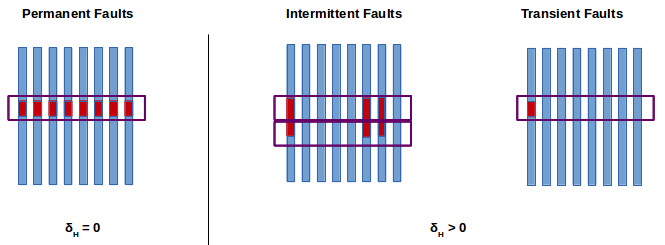
\includegraphics[scale=1.00]{figures/deltah.png}
    \caption{Expected behavior of $\delta_H$ for different faults}
    \label{fig:deltah}
  \end{center}
\end{figure}


\subsection{Resemblance of output cones}

\subsection{Diagnostic features}


